%Custom Functions
\newcommand{\CompanyName}{TT} % update later

\documentclass[conference]{IEEEtran}
\IEEEoverridecommandlockouts
% The preceding line is only needed to identify funding in the first footnote. If that is unneeded, please comment it out.
%\usepackage{cite}
\usepackage{amsmath,amssymb,amsfonts}
\usepackage{algorithmic}
\usepackage{graphicx}
\usepackage{textcomp}
\usepackage{xcolor}

\usepackage{pdflscape}

\usepackage[utf8]{inputenc}
\usepackage{fancyhdr}
\usepackage{lastpage}

% Please add the following required packages to your document preamble:
\usepackage{multirow}
\usepackage[numbers]{natbib}

\usepackage{listings}
\usepackage{hyperref}
\usepackage{amsmath}

\hypersetup{
    citecolor=black,
    colorlinks=true,
    linkcolor=black,
    filecolor=magenta,      
	urlcolor=cyan
}

\usepackage{listings}
\usepackage{color}

\definecolor{dkgreen}{rgb}{0,0.6,0}
\definecolor{gray}{rgb}{0.5,0.5,0.5}
\definecolor{mauve}{rgb}{0.58,0,0.82}

\lstset{frame=single,
  language=C++,
  showstringspaces=false,
  columns=flexible,
  basicstyle={\small\ttfamily},
  numbers = none,
  numberstyle=\tiny\color{gray},
  keywordstyle=\color{blue},
  commentstyle=\color{dkgreen},
  stringstyle=\color{mauve},
  breaklines=true,
  breakatwhitespace=true,
  tabsize=2
}

\def\BibTeX{{\rm B\kern-.05em{\sc i\kern-.025em b}\kern-.08em
T\kern-.1667em\lower.7ex\hbox{E}\kern-.125emX}}

\fancypagestyle{fancylandscape}{
\fancyhf{} %Clears the header/footer
\fancyfoot{% Footer
\makebox[\textwidth][r]{% Right
  \rlap{\hspace{.75cm}% Push out of margin by \footskip
    \smash{% Remove vertical height
      \raisebox{4.87in}{% Raise vertically
        \rotatebox{90}{Page \thepage\ of \pageref{LastPage}}}}}}}% Rotate counter-clockwise
\renewcommand{\headrulewidth}{0pt}% No header rule
\renewcommand{\footrulewidth}{0pt}% No footer rule
}

\pagestyle{fancyplain}
\fancyhf{}
\fancyfoot[c]{Page \thepage\ of \pageref{LastPage}}
\renewcommand{\headrulewidth}{0pt}

\begin{document}

	\title{Artificial Intelligence and Machine Learning: Search and ML Clustering}

	\author{\IEEEauthorblockN{1\textsuperscript{st} Given Edward Patch}
	\IEEEauthorblockA{\textit{Software Engineer (of BSc Year 3)} \\
    \textit{Artificial Intelligence and Machine Learning}\\
    \textit{University of Wales Trinity St. Davids (of Gordon Dickers)}\\
    Swansea, Wales \\
    Student ID: 1801492}}

     \maketitle
    
    \thispagestyle{plain}
    \pagestyle{plain}
    
    \begin{abstract}
      
    \end{abstract}

    \begin{IEEEkeywords}
      Deep First Search, KMeans, Algorithms.
    \end{IEEEkeywords}

    \section{Introduction}
      Artificial Intelligence (AI), commonly known as Machine Learning (ML), are built-up with many algorithms to provide tools to create AI and ML solutions. Research and implementation of two algorithms, Depth First Search and KMeans, to solve two given problems found within AI development.

      AI algorithms enable the developer to reuse algorithms to identify different items, generally in a recursive state. For instance, if a text file with the text stored as `Find me' was mixed with many other duplicate text files, then different algorithms could find precise information, whether it is a date and time or author's name from the file's metadata, creating a new identity to the found file.

    \section{Depth First Search}
      % Research
      DFS algorithm provides a method of finding a node through a tree-based search using a Stack data structure. The data structure stores new memory on top of recent memory within the Stack. A Stack only allows access to the last data added to the Stack. The algorithm selects the first node that is pre-identified before the algorithm starts. After this step, the algorithm will loop through each node, adding the latest node to the Stack, and if the node has no other pathways, the algorithm pops each node until the following path becomes available. This recursion continues until the finding of the search node. Although, if a particular node does not exist, the algorithm will not break, causing an infinite loop unless there is a `depth' variable. The process of the DFS algorithm summarised by Vigneshwaran Palanisamy's~\cite{palanisamy_novel_2020}, Journal Article, `A Novel Agent Based Depth First Search Algorithm' as quoted `DFS is about to start a source vertex s and travel the graph level by level, and it first visits all vertices which are adjacent to the s [5].' The time complexity of the DFS algorithm according to Vigneshwaran Palanisamy~\cite{palanisamy_novel_2020} `...DFS will be $\mathcal{O}(\mathcal{V}+\mathcal{E})$, where $\mathcal{V}$ is the number of vertices and $\mathcal{E}$ is the number of Edges.' It also states that if a matrix data structure is present, then it is noteworthy to measure the time complexity as $\mathcal{O}(\mathcal{V}^2)$.
      
      Dijkstra algorithm applies the Breadth-First Search (BFS) algorithm logic. The BFS algorithm functions with Queues rather than a Stack data structure. When the next available pathway becomes available, an addition of the following pathway to the queue's end, so when the objective node is not present, the algorithm will continue to the subsequent nodes on the next queue. Vigneshwaran Palanisamy~\cite{palanisamy_cluster_2020}, `Cluster Based Multi Agent System for Breadth First Search' mentions the time complexity of the Breadth-First Search is $\mathcal{O}(\mathcal{V} + \mathcal{E})$. Again, if the data structure uses a matrix data structure, then the time complexity is equal to $\mathcal{O}(\mathcal{V}^2)$.
            
      Dijkstra algorithm appears in different scenarios like AI pathfinding found in-game scenarios, where the enemy character tries finding the shortest pathway to find the main character. These algorithms weigh each pathway and select the best pathway that costs less time to complete. Instead of using queues, the Dijkstra algorithm uses weighted graphs to calculate the shortest path. According to `A Note on the Complexity of Dijkstra`s Algorithm for Graphs with Weighted Vertices' written by Michael Barbehenn~\cite{barbehenn_note_1998} `Therefore, the complexity of Dijkstra’s algorithm for vertex-based cost functions is $\mathcal{O}(|\mathcal{E}| + |\mathcal{V}| \log |\mathcal{V}|)$ using a binary
      heap implementation for the priority queue.' 

      Comparing the previously noted time complexities of DFS, BFS and Dijkstra algorithms, the following formulae offers an idea of how to calculate the time of completion for each one.
      \begin{center}
        \textbf{Time Complexities Formulae}\\
        \textit{$\mathcal{V}$:} Vertices | \textit{$\mathcal{E}$:} Edges

        \textbf{DFS:} $\mathcal{O}(\mathcal{V} + \mathcal{E})$\\
        \textbf{BFS:} $\mathcal{O}(\mathcal{V} + \mathcal{E})$\\
        \textbf{Dijkstra:} $\mathcal{O}(\mathcal{V} + \mathcal{E}(\log\mathcal{V}))$
      \end{center}

      With ${\mathcal{E} = 8}$ and $\mathcal{V} = 6$, DFS and BFS algorithms calculates to the time complexity of $\mathcal{O}(14)$ and Dijkstra algorithm is equal to the time complexity of $\mathcal{O}(13.42)$ rounded-up by two decimal places. DFS and BFS algorithms have similar execution times based solely on the time complexity. Dijkstra algorithm has a time complexity difference of $\mathcal{O}(0.58)$ compared to either DFS or BFS algorithms. However, due to the BFS algorithm being more memory intensive, the DFS algorithm will empty memory to find the next available pathway. This reasoning proves that even though both have the same time complexity, the BFS algorithm may prove slower than the DFS algorithm if the BFS algorithm causes the system memory to clog up. However, the BFS algorithm could prove quicker than the DFS algorithm if an infinite loop occurs.

      % Experiment
      The environment consists of several rules for the DFS algorithm to follow. This environment creates a test environment to provide different scenarios for the DFS algorithm implementation. These rules consist of:-
      \begin{itemize}
        \item C++ Programming Language.
        \item An ability to load different files with dynamic height and width.
        \item Ascii `42' characters are out-of-bounds.
        \item Ascii `32' characters are pathways.
        \item Ascii `83' character is a start position.
        \item Ascii `70' character is a finish position.
        \item Ascii `48 - 57 and 65 to 90' characters are nodes.
        \item Stack data structure to repsresent a DFS algorithm setup.
      \end{itemize}

      % Actual Results
      \textbf{Note:} The input file to test the DFS algorithm implementation is ‘m1.txt’, and the assignment of the search node is ‘E’. The content of the input file, figure~\ref{lstlisting:dfsInput}, page~\pageref{lstlisting:dfsInput}. Results of the DFS algorithm console logs found within figure~\ref{lstlisting:dfsApplicationResults}, page~\pageref{lstlisting:dfsApplicationResults}. Graph Results using MATLAB to plot the data from the CVS file generated the DFS implementation. MATLAB DFS application enables the user to control the depth to see the program's visualisation. Check out Figure~\ref{fig:dfsMatlabGraph}, page~\pageref{fig:dfsMatlabGraph}.
      \begin{figure}[h]
        \begin{lstlisting}[columns=fixed]
                  ***********
                  *S    A   *
                  ***** *****
                  *C*       *
                  * ******* *
                  * *       *
                  * ** ******
                  * *B     D*
                  * **** ** *
                  *E       F*
                  ***********
        \end{lstlisting}
        \caption{DFS Algorithm: Input File}
        \label{lstlisting:dfsInput}
      \end{figure}

      \begin{figure}[ht]
        \begin{lstlisting}[columns=fixed]
          Enter filename: m1.txt
          Enter Node to Find (Char): E
          ***********
          *S    A   *
          ***** *****
          *C*       *
          * ******* *
          * *       *
          * ** ******
          * *B     D*
          * **** ** *
          *E       F*
          **********
          N: S X: 1 | Y: 1 | Last Direction Enum: 0 | Current Direction Enum: 0
          N: A X: 1 | Y: 6 | Last Direction Enum: 1 | Current Direction Enum: 1
          N: S X: 1 | Y: 1 | Last Direction Enum: 0 | Current Direction Enum: 5
          N: B X: 7 | Y: 3 | Last Direction Enum: 3 | Current Direction Enum: 5
          N: E X: 9 | Y: 1 | Last Direction Enum: 3 | Current Direction Enum: 5
          Generated Necessary Data Files for Matlab:
          Go to the DFSMatlab folder and open DFS Matlab application
        \end{lstlisting}
        \caption{DFS Algorithm: Application Results}
        \label{lstlisting:dfsApplicationResults}
      \end{figure}

      \begin{figure}[ht]
        \centering
        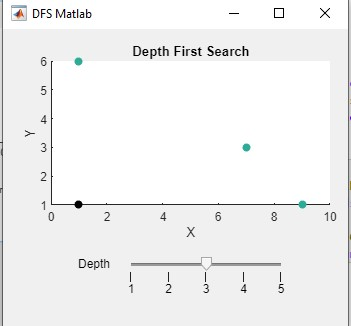
\includegraphics[width=0.65\columnwidth]{Figures/fig3.jpg}
        \caption{DFS Matlab Graph}
        \label{fig:dfsMatlabGraph}
      \end{figure}

    \section{KMeans}
      % Add mathematical formula for KCluster and Data Point sets.
      \begin{center}
        \textbf{The resprentation of the KMeans algorithm}
        \[ \mathcal{C}(n) = \left| 
        \begin{array}{ccc}
          \mathcal{K} & \mathcal{X} & \mathcal{Y}
        \end{array} \right|
        \]
        \[ \mathcal{K}(n \mathcal{<} \overline{\mathcal{C}}\frac{1}{2}) = \left| \begin{array}{cc}
          \mathcal{X} & \mathcal{Y}
          \end{array} \right|
        \] 

        $\sum_{\mathcal{C}_{n-1} \neq \mathcal{C}}^{\infty}$

        $\int_{\overline{\mathcal{C}}}^{i} \, \mathcal{C}_{ik}=
            _{\int_{\overline{\mathcal{K}}}^{j}  \,
              _{\left(\sqrt{(\mathcal{K}_{j x} - \mathcal{C}_{i x})^2 + \mathcal{K}_{j y} - \mathcal{C}_{iy})^2 }
              \right) \leq \mathcal{K}_{j}}}$

        $\int_{\overline{\mathcal{K}}}^{i} \,
        _{\left(\int_{\overline{\mathcal{C}}}^{j} \,
        _{\left(
          \mathcal{K}_{ij} =
         _{\left(\int_{2}{j} \, 
         \overline{\mathcal{M}_k} = \frac{\sum \mathcal{C}_{j \equiv i}^k}{n} 
         \right)}
        \right)}
        \mathcal{K}_{ik} =
        _{\left(\int_{\overline{\mathcal{M}}}^{j} \, 
          _{\left(\int_{2}^{k} \, 
            \mathcal{M}_{jk}
          \right)}
          \right)}
        \right)}$
        
      \end{center}

      KMeans, an unsupervised learning algorithm, works by sorting a given set of data points ($\mathcal{C}$) with a given size of K cluster points ($\mathcal{K}$) with a constraint of K length is less than half of $\mathcal{C}$ length. A random Center of Gravity (CoG) to each K cluster is assigned. This technique enables the software to start the grouping procedure. Based on the Journal Article, `Web User Clustering Analysis based on KMeans Algorithm', authored by JinHuaXu~\cite{jinhuaxu_web_2010} states that `These centroids should be placed in a cunning way because of different location causes different result. So, the better choice is to place them as much as possible far away from each other.' A way of fabricating this method into our implementation is to run a K Cluster through the randomise function; if a K Cluster $(\mathcal{X} \vee \mathcal{Y})$ CoG is the same, then randomise both $(\mathcal{X} \wedge  \mathcal{Y})$ on the K Cluster points again.

      After generating the data clusters and K clusters, the next stage determines which data points belong to which cluster. To do this, it is a matter of finding the distance. The formula used to solve this problem, $\left||\mathcal{C} - \mathcal{K}\right||$.
    \section{Visualisation Tools}

    \section{Terminology}
      List of terminologies used in this document:-
      \begin{itemize}
        \item AI - Artificial Intelligence.
        \item BFS - Breadth First Search.
        \item DFS - Depth First Search.
        \item ML - Machine Learning.
      \end{itemize}

    \section{Appendices}
      One of the ways to plot the data in steps within the MATLAB environment within the K-Means algorithm process was creating a C-library that communicates with existing code. This process enables users to interact with the MATLAB Application, changing data and watching the application plot. 
      
      Using the MathWorks - MATLAB Documentation, the library CLib successfully compile communication files and load EntryPoint functions. However, this method had another problem that proved time-consuming that consists of moving a \textit{string} over from the Clang to MATLAB. This was tried with, but not limited to, \textit{char*} and \textit{char[]} datatypes, referring to this manual~\url{https://uk.mathworks.com/help/matlab/matlab_external/passing-arguments-to-shared-library-functions.html}. 

      Below is some evidencing of the test library, communicating to the \textit{MTools} namespace, \textit{Randomise} function that generates a number within a range, using an argument of a C Struct with the name of `A'.
      
      \begin{figure}[ht]
        \centering
        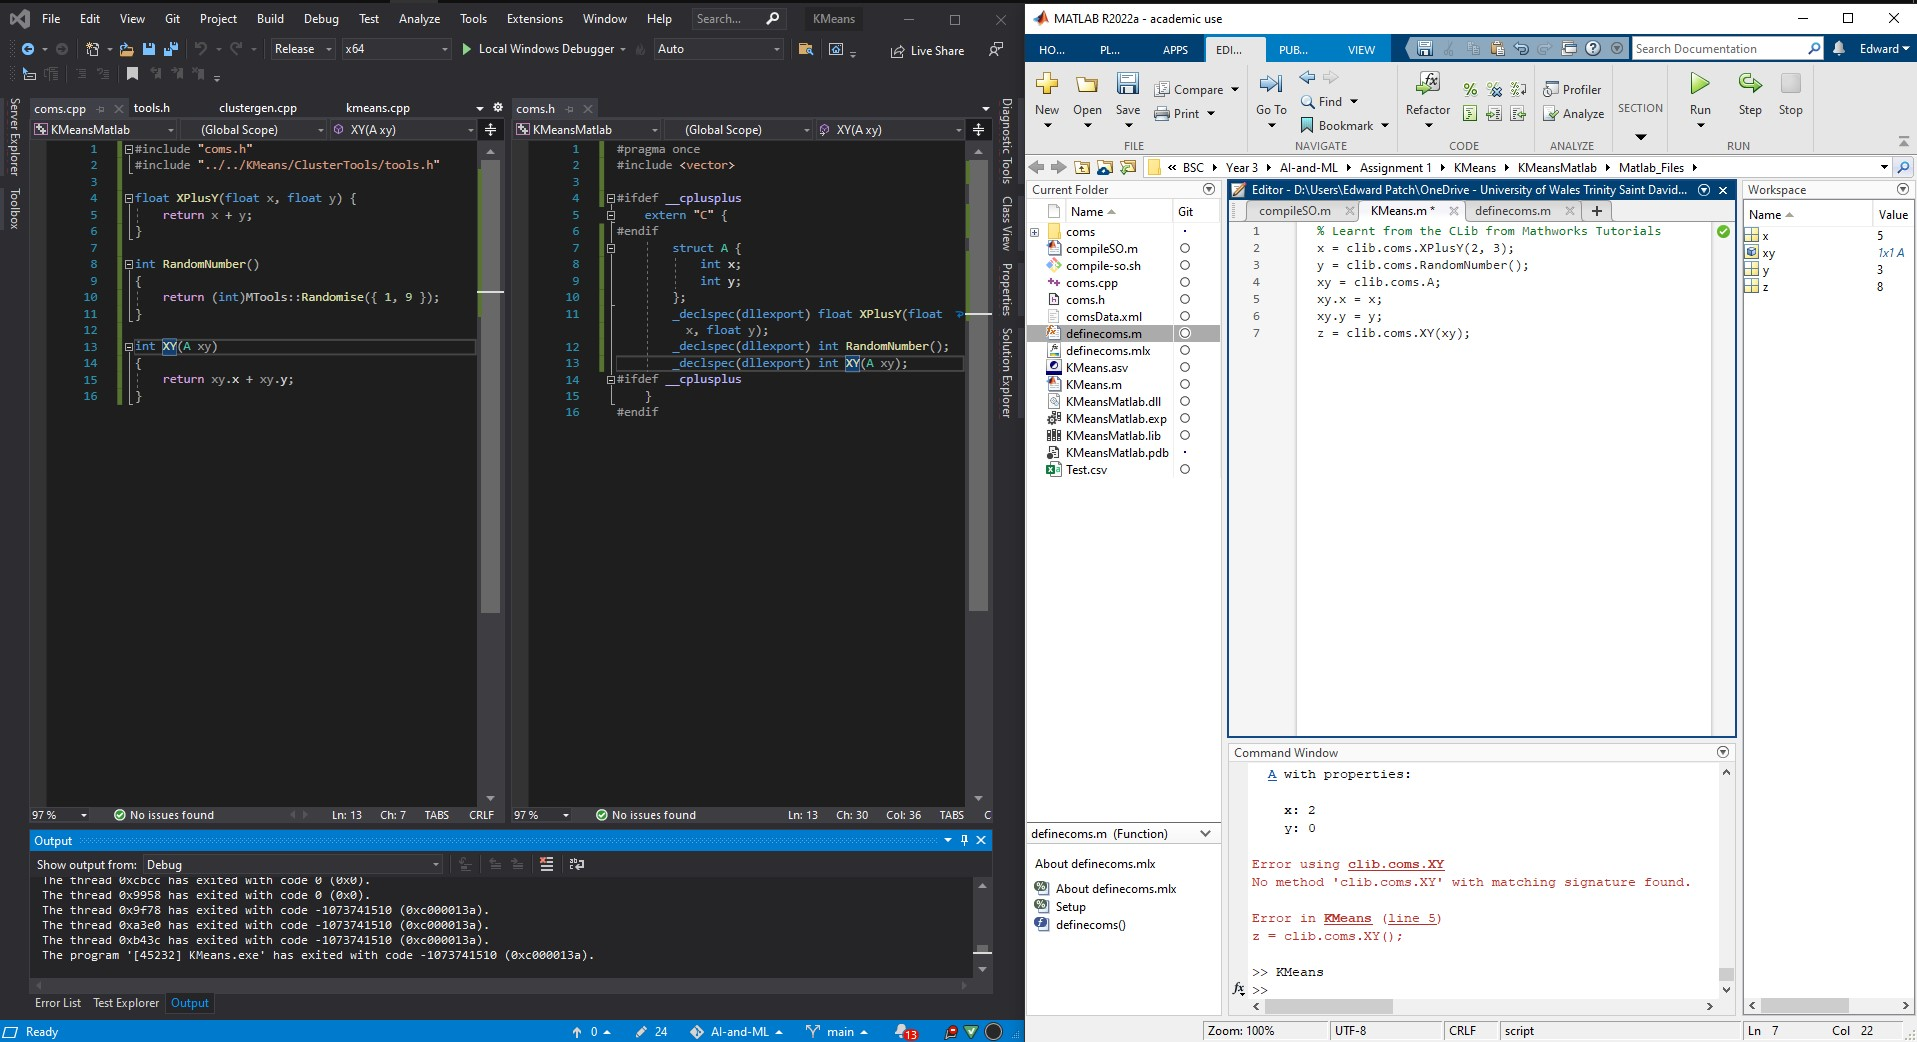
\includegraphics[width=1\columnwidth]{Figures/fig1.jpg}
        \caption{C and MATLAB Working}
        \label{fig:throughput}
      \end{figure}

      A updated version of the code and with an attempt to send strings over from MATLAB to the C lang.

      \textbf{Header:}
      \begin{lstlisting}[language=c]
        #pragma once

        #ifdef __WIN32
          #define EXPORT _declspec(dllexport)
        #else
          #define EXPORT
        #endif

        #ifdef __cplusplus
          extern "C" {
        #endif
          struct CMemory {
            char name*;
            int value;
          };

          namespace CreateData {
            EXPORT CMemory CreateCMemory(char *name, int size);
          }

        #ifdef __cplusplus
          }
        #endif
      \end{lstlisting}

      \textbf{Source:}
      \begin{lstlisting}[language=c++]
        #include "coms.h"

        CMemory CreateData::CreateCMemory(char *name, int size)
        {
            CMemory test({name, size});

            return test;
        }
      \end{lstlisting}
  \nocite{*}
	\renewcommand\refname{\section{Reference List}}
	\small{\bibliographystyle{IEEEtran}
    \bibliography{ref}}
\end{document}